\documentclass[runningheads,orivec]{llncs} 
\usepackage{amsmath,amssymb,mathtools}
\usepackage{enumitem}
\usepackage{hyperref}
\usepackage{microtype}
\usepackage[T1]{fontenc}
\usepackage{booktabs}
% Figures (message-flow)
\usepackage{tikz}
\usetikzlibrary{calc,arrows.meta,positioning}
\setlist[enumerate]{leftmargin=*,itemsep=0.25em}
% Algorithm boxes
\usepackage{algorithm}
\usepackage[noend]{algpseudocode}
\usepackage[section]{placeins}
\usepackage{float} % for H when absolutely needed
% dark PDF theme
\usepackage{xcolor}
\pagecolor[rgb]{0,0,0} %black
\color[rgb]{0.8,0.8,0.8} %grey

\newcommand{\prot}{\textsf{QuanTEEum}}
\newcommand{\sid}{\mathsf{sid}}
\newcommand{\Att}{\mathsf{AttestDelete}}
\newcommand{\RA}{\mathsf{RA}}
\newcommand{\FROST}{\textsf{FROST}}
\newcommand{\oss}{\textsf{OSS}}
\newcommand{\code}[1]{\texttt{#1}}

\begin{document}
\title{Short Paper: QuanTEEum: Quantum Cryptography via TEEs}
\author{[Redacted for review]}
\authorrunning{[Redacted for review]}
\institute{[Redacted for review]}
% \author{Shoaib Ahmed}
% \authorrunning{S. Ahmed}
% \institute{Independent Researcher\\ \email{sufialhussaini@gmail.com}}
\maketitle

\begin{abstract}
One-shot signatures (OSS) have emerged as a versatile abstraction underpinning various blockchain-facing applications. Existing OSS constructions rely on quantum hardware that will not be widely available soon. Naïve emulations using a single trusted execution environment (TEE) inherit brittle unclonability requirements and concentrate integrity risk in one enclave, while certified deletion on a single device is notoriously hard. 

We present \prot{}, an honest-minority distributed protocol that realizes certified deletion and OSS by running threshold signing entirely \emph{inside} heterogeneous TEEs. In \prot{}, $n$ enclaves run a threshold DKG, produce exactly one threshold signature on the designated message $m^{\star}$, and each emits a remote attestation (RA) binding an in-enclave deletion event; security is \emph{additive}, as independent deletion attestations strictly raise the minimum cost-of-attack, and TEE heterogeneity provides defense-in-depth against supply-chain risks. We formalize the \emph{exact-one} acceptance condition for one-shot signing in a remote attestation model under an abstract replay predicate \textsf{Fresh} (enforcing per-session counter monotonicity), and we \emph{discuss} pluggable attestation back ends—(a) conventional TEE RA, (b) cryptoeconomic attestations via escrowed collateral, and (c) future quantum instantiations—yielding a clean upgrade path. We sketch applications to QuanTEEum money and de-facto ceremony-free Groth16 CRS generation, and discuss liveness, freshness, and rollback subtleties. 
\end{abstract}

\section{Introduction}
\paragraph{Motivation.}
One-shot signatures (OSS) guarantee that a secret signing key can produce at most one valid signature; thereafter any further signing with that key is infeasible. Certified deletion complements OSS by providing verifiable deletion of the relevant secrets after use. Together, these primitives enable applications such as quantum money, perfect-finality blockchains, smart contracts without a blockchain, ordered and budgeted signatures, and ceremony-free Groth16 CRS. 
Current TEE-based attempts at realizing OSS typically use a single enclave, making certified deletion both hard and brittle. The central tension is that \emph{unclonability} pushes toward keeping a single non-replicated secret, whereas \emph{robustness and defense-in-depth} call for replication across heterogeneous TEEs. While supply chain hardening and reproducible builds are crucial, defense-in-depth via \emph{heterogeneous} enclaves gives additive security.
This motivates a design that achieves exact-once semantics while distributing trust across multiple enclaves.

\paragraph{Our approach.}
\prot{} lifts OSS to an \emph{honest-minority} setting by distributing the signing key across independent (heterogeneous) enclaves via a threshold DKG and binding the resulting (group) public key with per-enclave DKG attestations. The system produces exactly one threshold signature on the designated message and then aggregates per-enclave certified-deletion attestations bound to the same session. 
Exact-once acceptance reduces to the infeasibility of recovering a deleted threshold share from \emph{at least one} honest enclave, plus freshness/anti-replay for attestations and standard threshold unforgeability. We adopt the \emph{relaxed OSS} notion: one-shotness today via TEE-backed certified deletion, with a clean upgrade path to quantum implementations.

\paragraph{Contributions.}
\begin{itemize}[leftmargin=*,itemsep=0.25em,topsep=0.25em]
  \item A formalization of the \emph{exact-one} acceptance condition for one-shot signing in a remote attestation model with explicit context binding, parameterized by an abstract freshness predicate \textsf{Fresh}.
  \item \prot{}: a DKG-first threshold-in-TEE protocol that yields \emph{exactly one} threshold signature on a designated message and a set of per-enclave deletion attestations; security is additive across heterogeneous TEEs.
  \item A verifier-facing artifact and algorithm: the \emph{attested one-shot certificate} $\mathsf{AOSC}_\sid$ and \emph{VerifyAOSC}, enabling third-party validation under \textsf{Fresh}.
  \item Application sketches for (i) QuanTEEum money (quantum-money–flavored tokens) and (ii) de-facto ceremony-free Groth16 CRS via certified deletion.
  \item A discussion of liveness under abort, anti-replay/rollback resistance, policy-driven heterogeneity as defense-in-depth, and on-chain instantiation/incentives.
\end{itemize}

\section{Background and Model}
\subsection{One-shot signatures in brief}
A one-shot signature scheme \cite{amos2020one} is a tuple $(\mathsf{Gen},\mathsf{Sign},\mathsf{Ver})$ with syntax:
\[
\mathsf{Gen}(\mathsf{crs}) \rightarrow (pk,sk),\qquad
\mathsf{Sign}(sk,m) \rightarrow \sigma,\qquad
\mathsf{Ver}(\mathsf{crs},pk,m,\sigma) \rightarrow b \in \{0,1\}.
\]
\emph{Correctness:} if $(pk,sk) \leftarrow \mathsf{Gen}(\mathsf{crs})$ and $\sigma \leftarrow \mathsf{Sign}(sk,m)$ then $\mathsf{Ver}(\mathsf{crs},pk,m,\sigma)=1$. 

\smallskip
\noindent\emph{One-shot unforgeability:} no probabilistic polynomial-time (PPT) adversary, given $(\mathsf{crs},pk)$ and oracle access to $\mathsf{Sign}(sk,\cdot)$, can output two distinct valid pairs $(m_1,\sigma_1)\neq(m_2,\sigma_2)$ with $\mathsf{Ver}(\mathsf{crs},pk,m_1,\sigma_1)=\mathsf{Ver}(\mathsf{crs},pk,m_2,\sigma_2)=1$ except with negligible probability.

\smallskip
\noindent\emph{Remarks.} In our instantiation, the public parameters $\mathsf{crs}$ are absorbed into the suite/policy (Section~\ref{sec:protocol}); the secret key is classical but confined to TEEs. 

\subsection{Threshold signatures}
We assume a Schnorr-style $t$-of-$n$ threshold signature with a secure DKG (e.g., FROST~\cite{komlo2020frost}), where $n$ is the number of participating enclaves and $t$ is the signing threshold. Each party $P_i$ holds an additive secret share $sk_i$; together they define the group public key $pk$, and interactive signing with fresh per-round nonces from any set of $t$ parties produces signature $\sigma$ on message $m$. Security assumes a correct DKG, fewer than $t$ shares exposed, and no nonce reuse or bias. We primarily instantiate $t{=}n$; the case $t{<}n$ is discussed in \S\ref{sec:discussion}.

\subsection{TEE trust and remote attestation}
Each party $P_i$ hosts an enclave $E_i$ implementing \prot{}. We assume:
\begin{itemize}[leftmargin=*,itemsep=0.25em]
  \item \textbf{Code identity}: attestation binds a code measurement and the \emph{auxiliary reportdata} to outputs; verifier policy is committed via $\mathsf{policy\_hash}$ in $\mathsf{sid}$.
  \item \textbf{Sealed state semantics}: used only pre-signing to persist the DKG result across a crash.
  \item \textbf{Freshness/anti-replay}: a monotonic \emph{counter} is available (hardware counter or external append-only anchor) and is bound into attestations as $\mathsf{ctr}\in\{0,1,2\}$ corresponding to JOIN, DKG, and DEL.
  \item \textbf{Deletion API}: an enclave can make shares unrecoverable (\emph{zeroization}) and prove the transition with an attestation carrying auxiliary data.
\end{itemize}
We \emph{do not} assume perfect side-channel resistance or that all rollback vectors are impossible; instead we bind acceptance to the \emph{freshness predicate} and to a one-shot latch.

\paragraph{Assumption (Replay protection \textsf{Fresh}).}
There exists a predicate $\textsf{Fresh}(\mathsf{RA},\mathsf{sid})\!\in\!\{0,1\}$ enforcing per-$(\mathsf{sid},\mathsf{eid})$ \emph{uniqueness} and \emph{strict counter monotonicity} $0\!\rightarrow\!1\!\rightarrow\!2$. The verifier accepts at most one quote for each $(\mathsf{sid},\mathsf{eid},\mathsf{ctr})$, and any $\mathsf{ctr}{=}2$ (DEL) must be fresh relative to previously accepted $\mathsf{ctr}\in\{0,1\}$. No trusted time is required; realizations include enclave-backed monotonic storage or an external append-only anchor.

\subsection{Adversary and network}
The network is asynchronous with eventual delivery; the adversary may delay, drop, reorder, and duplicate messages. Channels are authenticated and confidential (RA--TLS). The adversary is rushing and may statically corrupt up to $f$ enclaves and their hosts. We target $t{=}n$ for strongest one-shot semantics; extensions to $t<n$ are discussed in \S\ref{sec:discussion}.

\section{\prot{} Protocol}\label{sec:protocol}

\begin{figure}[!htbp]
\centering
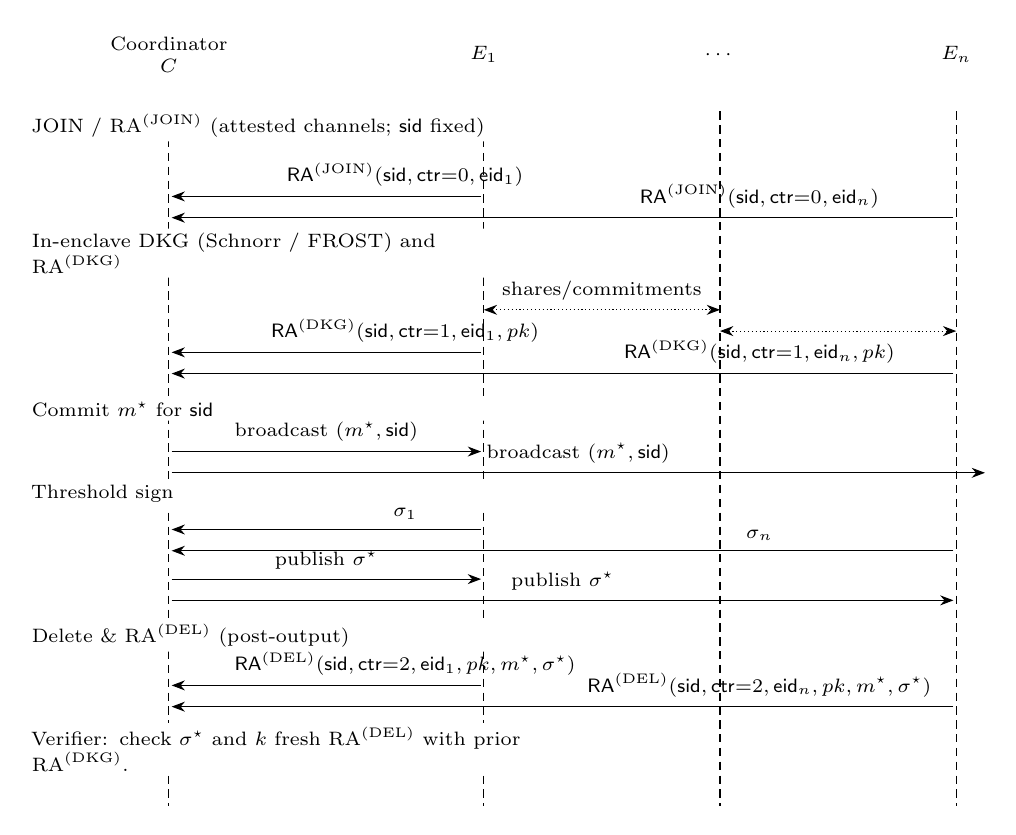
\begin{tikzpicture}[
  x=2.0cm,y=0.9cm,>=Stealth,
  every node/.style={font=\scriptsize},
  msg/.style={->,line width=0.4pt,shorten >=1pt,shorten <=1pt},
  lifeline/.style={densely dashed,line width=0.4pt},
  ann/.style={anchor=west,fill=white,inner sep=1.5pt,rounded corners=1pt,text width=6.2cm}
]
  % Column labels (kept separate from lifeline anchors)
  \node[align=center] (C_lbl)  at (0,0)   {Coordinator\\$C$};
  \node[align=center] (E1_lbl) at (2,0)   {$E_1$};
  \node[align=center] (Ed_lbl) at (3.5,0) {$\cdots$};
  \node[align=center] (En_lbl) at (5,0)   {$E_n$};

  % Lifeline anchors start below labels to avoid overlap
  \coordinate (C)  at (0,-0.8);
  \coordinate (E1) at (2,-0.8);
  \coordinate (Ed) at (3.5,-0.8);
  \coordinate (En) at (5,-0.8);

  % Lifelines
  \draw[lifeline] (C)  -- +(0,-9.8);
  \draw[lifeline] (E1) -- +(0,-9.8);
  \draw[lifeline] (Ed) -- +(0,-9.8);
  \draw[lifeline] (En) -- +(0,-9.8);

  % LEFT-MARGIN ANNOTATIONS (white boxes) to avoid any overlap with arrows
  \node[ann] at (-0.9,-1.0) {JOIN / RA$^{(\mathrm{JOIN})}$ (attested channels; $\mathsf{sid}$ fixed)};
  \node[ann] at (-0.9,-2.8) {In-enclave DKG (Schnorr / FROST) and RA$^{(\mathrm{DKG})}$};
  \node[ann] at (-0.9,-5.0) {Commit $m^{\star}$ for $\mathsf{sid}$};
  \node[ann] at (-0.9,-6.2) {Threshold sign};
  \node[ann] at (-0.9,-8.2) {Delete \& RA$^{(\mathrm{DEL})}$ (post-output)};
  \node[ann] at (-0.9,-9.8) {Verifier: check $\sigma^{\star}$ and $k$ fresh RA$^{(\mathrm{DEL})}$ with prior RA$^{(\mathrm{DKG})}$.};

  % 1) JOIN / RA^{(JOIN)}
  \draw[msg] ($(E1)+(0,-1.2)$) -- node[above,sloped,near start]{$\RA^{(\mathrm{JOIN})}(\mathsf{sid},\mathsf{ctr}{=}0,\mathsf{eid}_1)$} ($(C)+(0,-1.2)$);
  \draw[msg] ($(En)+(0,-1.5)$) -- node[above,sloped,near start]{$\RA^{(\mathrm{JOIN})}(\mathsf{sid},\mathsf{ctr}{=}0,\mathsf{eid}_n)$} ($(C)+(0,-1.5)$);

  % 2) DKG (peer-to-peer) + RA^{(DKG)}
  \draw[<->,densely dotted,line width=0.4pt] ($(E1)+(0,-2.8)$) -- node[above]{shares/commitments} ($(Ed)+(0,-2.8)$);
  \draw[<->,densely dotted,line width=0.4pt] ($(Ed)+(0,-3.1)$) -- ($(En)+(0,-3.1)$);
  \draw[msg] ($(E1)+(0,-3.4)$) -- node[above,sloped,near start]{$\RA^{(\mathrm{DKG})}(\mathsf{sid},\mathsf{ctr}{=}1,\mathsf{eid}_1,pk)$} ($(C)+(0,-3.4)$);
  \draw[msg] ($(En)+(0,-3.7)$) -- node[above,sloped,near start]{$\RA^{(\mathrm{DKG})}(\mathsf{sid},\mathsf{ctr}{=}1,\mathsf{eid}_n,pk)$} ($(C)+(0,-3.7)$);

  % 3) Commit (freeze message for this sid)
  \draw[msg] ($(C)+(0,-4.8)$) -- node[above,sloped]{broadcast $(m^{\star},\mathsf{sid})$} ($(E1)+(0,-4.8)$);
  \draw[msg] ($(C)+(0,-5.1)$) -- node[above,sloped]{broadcast $(m^{\star},\mathsf{sid})$} ($(En)+(0.2,-5.1)$);

  % 4) Sign (partials to aggregate)
  \draw[msg] ($(E1)+(0,-5.9)$) -- node[above,sloped,near start]{$\sigma_1$} ($(C)+(0,-5.9)$);
  \draw[msg] ($(En)+(0,-6.2)$) -- node[above,sloped,near start]{$\sigma_n$} ($(C)+(0,-6.2)$);
  \draw[msg] ($(C)+(0,-6.6)$) -- node[above,sloped]{publish $\sigma^{\star}$} ($(E1)+(0,-6.6)$);
  \draw[msg] ($(C)+(0,-6.9)$) -- node[above,sloped]{publish $\sigma^{\star}$} ($(En)+(0,-6.9)$);

  % 5) Certified deletion & RA^{(DEL)}
  \draw[msg] ($(E1)+(0,-8.1)$) -- node[above,sloped,near start]{$\RA^{(\mathrm{DEL})}(\mathsf{sid},\mathsf{ctr}{=}2,\mathsf{eid}_1,pk,m^{\star},\sigma^{\star})$} ($(C)+(0,-8.1)$);
  \draw[msg] ($(En)+(0,-8.4)$) -- node[above,sloped,near start]{$\RA^{(\mathrm{DEL})}(\mathsf{sid},\mathsf{ctr}{=}2,\mathsf{eid}_n,pk,m^{\star},\sigma^{\star})$} ($(C)+(0,-8.4)$);
\end{tikzpicture}
\caption{QuanTEEum message flow: RA$^{(\mathrm{JOIN})}$, RA$^{(\mathrm{DKG})}$ (bind $pk$), Commit $m^{\star}$, Sign, RA$^{(\mathrm{DEL})}$ (delete sk).}
\label{fig:flow}
\end{figure}

\paragraph{Roles.}
Parties $\{P_1,\dots,P_n\}$ run enclaves $\{E_1,\dots,E_n\}$.
A (rotating) coordinator $C$ orchestrates rounds but learns no secrets.
All protocol traffic (JOIN, DKG, Commit, Sign, Delete) is carried over
\emph{attested secure channels} (e.g., RA--TLS) whose channel binding includes an
ephemeral enclave public key $\mathsf{eid}$ attested by the enclave.

\paragraph{Session binding.}
We use DKG-first. A session identifier $\mathsf{sid}$ is derived
\[
  \mathsf{sid} \gets H(\mathsf{suite}\,\|\,\mathsf{policy\_hash}\,\|\,\mathsf{nonce}),
\]
and is embedded in all protocol messages and in the attestation \emph{reportdata}.
Here $\mathsf{nonce}$ is a fresh 128-bit value chosen by $C$ at JOIN.
The designated message $m^{\star}$ is \emph{frozen later} by a Commit step
(after DKG and before signing) and appears in the deletion attestation.

\paragraph{Parameters.}
\begin{itemize}[leftmargin=*,itemsep=0.25em]
  \item $\mathsf{suite}$: cryptographic suite identifier (curve/group, hash, domain separators, transcript encoding, threshold-signing variant).
  \item $\mathsf{policy}$: canonical verifier policy (e.g., $n,t$, minimum $\mathsf{DEL}$ attestations $k$, vendor/diversity constraints, RA roots, allowed measurements, freshness/replay-protection details).
  \item $\mathsf{policy\_hash} := H(\mathsf{policy})$ (committed by $\mathsf{sid}$).
  \item $\mathsf{nonce}$: 128-bit coordinator nonce ensuring $\mathsf{sid}$ uniqueness.
  \item $\mathsf{eid}$: enclave’s attested ephemeral DH/public key (per session), also used to bind the RA--TLS channel.
\end{itemize}

\paragraph{Attestation reportdata (aux).}
We use a \emph{monotonic counter} $\mathsf{ctr}\in\{0,1,2\}$ carried in the reportdata; no phase tags or timestamps.
All encodings are length-delimited and unambiguous.
\begin{align*}
  \text{RA}^{(\mathrm{JOIN})}\!:\ & \mathsf{aux} = (\mathsf{sid},\ \mathsf{ctr}{=}0,\ \mathsf{eid}) \\
  \text{RA}^{(\mathrm{DKG})}\!:\ & \mathsf{aux} = (\mathsf{sid},\ \mathsf{ctr}{=}1,\ \mathsf{eid},\ pk) \\
  \text{RA}^{(\mathrm{DEL})}\!:\ & \mathsf{aux} = (\mathsf{sid},\ \mathsf{ctr}{=}2,\ \mathsf{eid},\ pk,\ m^{\star},\ \sigma^{\star})
\end{align*}
Intuition: RA$^{(\mathrm{JOIN})}$ gates participation and binds $\mathsf{eid}$ to $\mathsf{sid}$; RA$^{(\mathsf{DKG})}$ binds the DKG result $pk$ to $\mathsf{sid}$ and $\mathsf{eid}$;
RA$^{(\mathrm{DEL})}$ certifies deletion \emph{after} producing the unique output $(m^{\star},\sigma^{\star})$.

\paragraph{Freshness and anti-replay.}
We rely on an abstract predicate $\textsf{Fresh}(\mathsf{RA},\mathsf{sid})$ that captures replay protection via either enclave-backed monotonic storage
or an external anchor (e.g., blockchain/notary). For each fixed $(\mathsf{sid},\mathsf{eid})$ the verifier accepts at most one quote per counter value and requires
strict monotonicity: any accepted $\mathsf{ctr}{=}2$ must be \emph{fresh} relative to any prior accepted $\mathsf{ctr}{\in}\{0,1\}$; duplicates or non-increasing counters are rejected.

\paragraph{Policy checks:}
\begin{description}
\item[\textbf{JOIN:}] $C$ sends $(\mathsf{suite},\mathsf{policy},\mathsf{nonce},\mathsf{sid})$ to the selected roster. Each enclave locally admits $\mathsf{policy}$ (e.g., allowlist or operator-signed), then emits RA$^{(\mathrm{JOIN})}$.
  $C$ proceeds only with enclaves whose RA$^{(\mathrm{JOIN})}$ verifies and whose $\mathsf{sid}$ matches.
  \item[\textbf{DKG:}] Enclaves run DKG over RA-bound channels; after DKG each emits RA$^{(\mathsf{DKG})}$ with $(\mathsf{sid},\mathsf{ctr}{=}1,\mathsf{eid},pk)$.
  $C$ ensures all RA$^{(\mathsf{DKG})}$ bind to the same $(\mathsf{sid},pk)$.
  \item[\textbf{Verification:}] An external verifier recomputes $\mathsf{policy\_hash}$ from its configured $\mathsf{policy}$,
  checks that $\mathsf{sid}$ commits to it, and accepts iff:
  \begin{enumerate}
    \item[(a)] $\mathsf{Verify}(pk,m^{\star},\sigma^{\star})=1$,
    \item[(b)] there are at least $k$ valid RA$^{(\mathrm{DEL})}$ with distinct $\mathsf{eid}$ satisfying diversity constraints, and
    \item[(c)] each such RA$^{(\mathrm{DEL})}$ is \emph{fresh}, i.e., $\textsf{Fresh}(\mathsf{RA}^{(\mathrm{DEL})},\mathsf{sid}){=}1$ and reflects strict counter increase relative to any previously accepted quotes for $(\mathsf{sid},\mathsf{eid})$ (JOIN optional, DKG precedes DEL).
  \end{enumerate}
\end{description}

\subsection*{Interfaces and notation}
\begin{itemize}[leftmargin=*,itemsep=0.25em]
  \item $\textsf{RA.GenQuote}(\mathsf{aux}) \rightarrow \mathsf{RA}$:
  produce a vendor-signed attestation over the enclave measurement and the byte string $\mathsf{aux}$.

  \item $\textsf{RA.Verify}(\mathsf{RA};\ \textsf{allow\_meas},\ \textsf{roots}) \in \{0,1\}$:
  verify signature under trusted RA roots and check the code measurement against the allowlist.

  \item $\textsf{Fresh}(\mathsf{RA},\mathsf{sid}) \in \{0,1\}$:
  abstract replay-protection predicate that enforces at most one accepted quote per $(\mathsf{sid},\mathsf{eid},\mathsf{ctr})$
  and strict counter monotonicity for $(\mathsf{sid},\mathsf{eid})$ across JOIN ($0$), DKG ($1$), and DEL ($2$).
  Instantiations include enclave-backed monotonic counters or an external append-only anchor.

  \item $\textsf{Latch}(\sid,m^{\star})$:
  bind $m^{\star}$ for this session inside the enclave; subsequent signing attempts under the same $\sid$ abort.

  \item $\textsf{Del}()$:
  irrecoverably zeroize the in-enclave key material and nonces (invoked before RA$^{(\mathrm{DEL})}$).
\end{itemize}

\subsection{Setup and DKG}
\emph{Algorithm~\ref{alg:setup} performs policy-based roster selection, attested JOIN with peer vetting, runs the in\mbox{-}enclave threshold DKG coordinated by $C$, and binds the group key via RA$^{(\mathrm{DKG})}$.}

\begin{algorithm}[!htbp]
\caption{\prot{}: \emph{SetupAndDKG}}
\label{alg:setup}
\begin{small}
\begin{algorithmic}[1]
\State $C$ selects a roster $R$ of enclaves satisfying $\mathsf{policy}$ (diversity, allowlisted measurements, RA roots) and sends $(\mathsf{suite},\mathsf{policy},\mathsf{nonce},\mathsf{sid})$ to all $E_i\in R$.
\For{each enclave $E_i\in R$}
  \State Measure code $\mathsf{meas}$; generate ephemeral $\mathsf{eid}_i$; establish RA--TLS channel bound to $\mathsf{eid}_i$.
  \State $\mathsf{RA}^{(\mathrm{JOIN})}_i \gets \textsf{RA.GenQuote}\big((\mathsf{sid},\mathsf{ctr}{=}0,\mathsf{eid}_i)\big)$; send to $C$.
\EndFor
\State $C$ distributes $\{\mathsf{RA}^{(\mathrm{JOIN})}_j\}_{j\in R}$ to all $E_i\in R$.
\For{each enclave $E_i\in R$ \textbf{in parallel}}
  \State For each $\mathsf{RA}^{(\mathrm{JOIN})}_j$: run \textsf{RA.Verify}; assert same $\mathsf{sid}$ and that the \emph{set} of participants satisfies $\mathsf{policy}$; abort on failure.
  \State Participate (over RA--TLS) in the in\mbox{-}enclave \emph{threshold DKG} coordinated by $C$ to derive local share $sk_i$ and common group $pk$; \textbf{never} export $sk_i$.
  \State $\mathsf{RA}^{(\mathrm{DKG})}_i \gets \textsf{RA.GenQuote}\big((\mathsf{sid},\mathsf{ctr}{=}1,\mathsf{eid}_i,pk)\big)$; send to $C$.
\EndFor
\State $C$ verifies all $\mathsf{RA}^{(\mathrm{DKG})}_i$ and that they bind to the same $(\mathsf{sid},pk)$; abort otherwise.
\State \textbf{return} $pk$ (to the application/coordinator).
\end{algorithmic}
\end{small}
\end{algorithm}

\subsection{Single-signing phase}
\emph{Algorithm~\ref{alg:sign} commits the designated message, latches it one-shot in each enclave, and performs threshold signing with $C$ aggregating.}

\begin{algorithm}[!htbp]
\caption{\prot{}: \emph{SingleSign} on designated message $m^{\star}$}
\label{alg:sign}
\begin{small}
\begin{algorithmic}[1]
\State $C$ broadcasts $(m^{\star},\mathsf{sid})$ over the RA--TLS channel (using the already-established $\mathsf{sid}$).
\For{each enclave $E_i$ \textbf{in parallel}}
  \State Check $\mathsf{sid}$ equality with local session; abort if mismatched or already latched.
  \State $\textsf{Latch}(\mathsf{sid},m^{\star})$ to bind the one-shot target (further signing under the same $\mathsf{sid}$ is refused).
  \State Run partial signing on $m^{\star}$ to obtain $\sigma_i$; send $\sigma_i$ to $C$ over RA--TLS.
\EndFor
\State $C$ aggregates $\{\sigma_i\}$ into $\sigma^{\star}$; \textbf{proceed to \emph{DeleteAndPublish}} (Alg.~\ref{alg:delete-publish}).
\end{algorithmic}
\end{small}
\end{algorithm}

\subsection{Certified deletion and publication}
\emph{Algorithm~\ref{alg:delete-publish} has $C$ request deletion attestations (including $\sigma^{\star}$) and enclaves attest deletion; $C$ then publishes the attested one-shot certificate $\mathsf{AOSC}_\sid$.}

\begin{algorithm}[!htbp]
\caption{\prot{}: \emph{DeleteAndPublish}}
\label{alg:delete-publish}
\begin{small}
\begin{algorithmic}[1]
\State \textbf{$C$} broadcasts over RA--TLS a deletion request containing $(\sid,pk,m^{\star},\sigma^{\star})$ to the session roster.
\For{each enclave $E_i$ \textbf{in parallel}}
  \State Receive $(\sid,pk,m^{\star},\sigma^{\star})$ over RA--TLS; check $\sid$ matches local session (abort on mismatch).
  \State \textsf{Del}(): zeroize local key material and nonces.
  \State $\mathsf{RA}^{(\mathrm{DEL})}_i \gets \textsf{RA.GenQuote}\big((\sid,\mathsf{ctr}{=}2,\mathsf{eid}_i,pk,m^{\star},\sigma^{\star})\big)$.
  \State Send $\mathsf{RA}^{(\mathrm{DEL})}_i$ to \textbf{$C$} over RA--TLS.
\EndFor
\State \textbf{$C$} initializes $S \gets \emptyset$.
\For{each enclave $E_i$}
  \State \textbf{$C$} receives $\mathsf{RA}^{(\mathrm{DEL})}_i$; add $(\mathsf{eid}_i,\mathsf{RA}^{(\mathrm{DEL})}_i)$ to $S$.
\EndFor
\State \textbf{$C$} chooses a policy-compliant subset $S' \subseteq S$ with $|S'|\ge k$.
\State \textbf{$C$ publishes} $\mathsf{AOSC}_\sid = (\sid,\mathsf{suite},\mathsf{policy\_hash},\mathsf{nonce},pk,m^{\star},\sigma^{\star},S')$.
\end{algorithmic}
\end{small}
\end{algorithm}

\paragraph{Output artifact (published by $C$).}
We define the \emph{attested one-shot certificate} for session $\sid$ as
\[
\mathsf{AOSC}_\sid := \big(\sid,\ \mathsf{suite},\ \mathsf{policy\_hash},\ \mathsf{nonce},\ pk,\ m^{\star},\ \sigma^{\star},\ \{(\mathsf{eid}_i,\ \mathsf{RA}^{(\mathrm{DEL})}_i)\}_{i\in S'}\big),
\]
where $S'$ is an index set with $|S'|\ge k$ satisfying the policy’s diversity constraints, and each
$\mathsf{RA}^{(\mathrm{DEL})}_i$ has $\mathsf{aux}=(\sid,\mathsf{ctr}{=}2,\mathsf{eid}_i,pk,m^{\star},\sigma^{\star})$.

\subsection{VerifyAOSC}
\emph{Algorithm~\ref{alg:verify-aosc} validates the published certificate against policy binding, signature correctness, and per-enclave RA freshness.}


\begin{algorithm}[!htbp]
\caption{\prot{}: \emph{VerifyAOSC}$(\mathsf{AOSC}_\sid)$}
\label{alg:verify-aosc}
\begin{small}
\begin{algorithmic}[1]
\State \textbf{Input:} $\mathsf{AOSC}_\sid = (\sid,\mathsf{suite},\mathsf{policy\_hash},\mathsf{nonce},pk,m^{\star},\sigma^{\star},\{(\mathsf{eid}_i,\mathsf{RA}^{(\mathrm{DEL})}_i)\}_{i\in S'})$
\State \textbf{Params:} trusted RA roots, allowed measurement set $\textsf{allow\_meas}$, policy (to rederive $\mathsf{policy\_hash}$ and diversity), freshness predicate \textsf{Fresh}
\State Recompute $\sid' \gets H(\mathsf{suite}\,\|\,\mathsf{policy\_hash}\,\|\,\mathsf{nonce})$ and assert $\sid'=\sid$
\State Assert $\mathsf{policy\_hash}$ matches the verifier’s configured policy; check $|S'|\ge k$ and diversity constraints on $\{\mathsf{eid}_i\}_{i\in S'}$
\State Check $\mathsf{Verify}(pk,m^{\star},\sigma^{\star})=1$
\For{each $i\in S'$}
  \State $\textbf{(a)}$ \textsf{RA.Verify}$(\mathsf{RA}^{(\mathrm{DEL})}_i;\ \textsf{allow\_meas},\ \text{RA roots})=1$
  \State $\textbf{(b)}$ Parse $\mathsf{aux}$ from $\mathsf{RA}^{(\mathrm{DEL})}_i$ and assert $\mathsf{aux}=(\sid,\mathsf{ctr}{=}2,\mathsf{eid}_i,pk,m^{\star},\sigma^{\star})$
  \State $\textbf{(c)}$ Ensure freshness: $\textsf{Fresh}(\mathsf{RA}^{(\mathrm{DEL})}_i,\sid)=1$ and strictly increasing counter vs.\ any prior accepted quotes for $(\sid,\mathsf{eid}_i)$
\EndFor
\State \textbf{Accept} iff all checks pass
\end{algorithmic}
\end{small}
\end{algorithm}

\noindent\emph{Note.} The above acceptance rule enforces the exact-one semantics; see Theorem~\ref{thm:one-shot}.

\section{Security}\label{sec:security}
We sketch the core arguments; full proofs follow standard game-hopping with an idealized \textsf{Fresh} predicate.
\paragraph{Safety: one-shot unforgeability.}
\begin{theorem}[One-shot from threshold-in-TEE]\label{thm:one-shot}
Assume (i) the underlying threshold signature is unforgeable, (ii) at least one enclave is honest and transitions to post-delete state after producing $\sigma^{\star}$, (iii) \textsf{Fresh} prevents replay/rollback of pre-delete states, and (iv) vendor RA is unforgeable under the stated trust roots. Then producing two distinct accepting artifacts for the same $pk$ in session $\mathsf{sid}$—i.e., two certificates that both pass \textsf{VerifyAOSC}—with $\sigma_1 \neq \sigma_2$ is infeasible for PPT adversaries.
\end{theorem}

\begin{proof}[Proof sketch]
Suppose two accepting artifacts exist. If either signature is produced without $t$ valid shares, we break threshold unforgeability. Otherwise, at least $t$ shares were live at each signing. Any accepting certificate contains at least $k$ valid deletion attestations, and under the honest-minority assumption at least one of those enclaves is honest and has deleted its share bound to $(\mathsf{sid},m^{\star},\sigma^{\star})$. The only routes to a second accepted signature are: (A) forge RA to claim deletion without deleting (contradicts RA unforgeability); (B) roll back an honest enclave past delete (contradicts \textsf{Fresh}); or (C) compromise enough enclaves (meeting policy/diversity constraints) to reassemble $t$ fresh shares (violates honest-minority).
\end{proof}

\paragraph{Liveness.}
With $t{=}n$ the protocol requires all enclaves to participate; a crashed or aborting enclave prevents progress. We adopt a bounded timeout: if signing fails, $C$ abandons $\sid$ and re-instantiates (fresh $\sid$ and DKG) with fresh enclaves. In deployments desiring partial progress, \prot{} supports $t<n$ with two caveats: (i) \emph{deletion} attestations must reach $k\!\ge\!t$; (ii) the exact-one property is now conditioned on at least one of the $k$ attesting enclaves being honest.

\paragraph{Additive security via heterogeneity.}
If attestations are independent across vendors/geographies/operators, the minimum cost\mbox{-}of\mbox{-}attack is approximately the sum of the $k$ cheapest per\mbox{-}enclave compromise costs (this approximation assumes independence and no bulk\mbox{-}attack economies; otherwise treat it as a lower bound). We recommend explicit \emph{diversity constraints} in policy (e.g., “at least two vendors and three physical operators”).

\paragraph{Freshness and anti-replay.}
Verifiers enforce an abstract replay predicate $\textsf{Fresh}$ rather than trusted time. For each $(\sid,\mathsf{eid})$, accept at most one attestation per counter value $\mathsf{ctr}\!\in\!\{0,1,2\}$ (JOIN, DKG, DEL) and require strict monotonicity $0\!\rightarrow\!1\!\rightarrow\!2$. Concretely, for every RA$^{(\mathrm{DEL})}$ in the certificate, check $\textsf{Fresh}(\mathsf{RA}^{(\mathrm{DEL})},\sid){=}1$ and that its $\mathsf{aux}$ binds $(\sid,\mathsf{ctr}{=}2,\mathsf{eid},pk,m^{\star},\sigma^{\star})$. Instantiations of $\textsf{Fresh}$ include enclave-backed monotonic storage or an external append-only anchor; no trusted timestamps are assumed.

\section{Applications}\label{sec:apps}

\subsection{\prot{} One-shot signatures (OSS)}\label{sec:app-oss}
\begin{itemize}[leftmargin=*,itemsep=0.25em]
  \item \textbf{KeyGen (\(\mathsf{Gen}(\mathsf{crs})\!\to\!(pk,sk)\)).} Instantiate a fresh \(\sid\); run \emph{SetupAndDKG} (Alg.~\ref{alg:setup}) to obtain \(pk\). The secret key \(sk\) is an opaque handle to the distributed in-enclave state for \(\sid\) (shares never leave TEEs).
  \item \textbf{Sign (\(\mathsf{Sign}(sk,m)\!\to\!\sigma\)).} Run \emph{SingleSign} (Alg.~\ref{alg:sign}) on \(m\) to obtain \(\sigma^{\star}\), then \emph{DeleteAndPublish} (Alg.~\ref{alg:delete-publish}) to get \(\mathsf{AOSC}_{\sid}\). Output \(\sigma := (\sigma^{\star}, \mathsf{AOSC}_{\sid})\).
  \item \textbf{Verify (\(\mathsf{Ver}(\mathsf{crs},pk,m,\sigma)\!\to\! b\)).} Parse \(\sigma=(\sigma^{\star},\mathsf{AOSC}_{\sid})\); accept (\(b{=}1\)) iff \(\mathsf{Verify}(pk,m,\sigma^{\star})=1\) and \emph{VerifyAOSC} (Alg.~\ref{alg:verify-aosc}) accepts \(\mathsf{AOSC}_{\sid}\).
\end{itemize}

\subsection{QuanTEEum money}
Following the OSS-based quantum money with \emph{classical} communication paradigm ~\cite{shmueli2025one}, a coin is a chain of one-shot signatures over successive recipients’ serials/keys: the mint signs Alice’s serial; on transfer, Alice one-shot signs Bob’s, and so on, so the previous signing capability self-destructs after each hop. \prot{} instantiates this with TEEs: each minting/transfer runs a fresh session to produce $(pk,\sigma^{\star},\mathsf{AOSC}_\sid)$ where $m^{\star}$ encodes the coin serial (and, if desired, the next recipient), and RA$^{(\mathrm{DEL})}$ certifies in-enclave key erasure. The “one-shot” effect we rely on is precisely that the signing key can be used only once (collapses thereafter).

\subsection{QuanTEEum ceremony-free CRS (Groth16)}
We specialize \prot{} to a \emph{distributed certified-deletion} workflow—no DKG, no signing—since a ceremony’s goal is only to ensure toxic waste is unrecoverable. For a circuit with identifier $\mathsf{cid}=H(\text{QAP})$, enclaves jointly compute the Groth16 CRS inside TEEs (deriving any trapdoor material ephemerally), publish the CRS, then zeroize and attest deletion. Concretely, we reuse JOIN (policy/roster, RA–bound channels), compute the CRS in-enclave, and have each enclave emit a deletion quote binding $(\sid,\mathsf{cid},H(\mathsf{CRS}))$. Verifiers accept a CRS iff at least $k$ deletion attestations validate and are fresh. This is not a plain-model proof of “no toxic waste,” but yields an auditable, honest-minority and heterogeneous alternative to single-operator ceremonies for Groth16.

\section{Discussion and Future Work}\label{sec:discussion}
\paragraph{Why $t\!=\!n$ first?}
It maximizes the exact-one semantics and simplifies acceptance (\emph{all} attest). Generalizing to $t<n$ is straightforward mechanically but shifts the trust statement to “among the $k\!\ge\!t$ attesters, at least one honest enclave deleted.”

\paragraph{Nonce discipline.}
Nonce misuse is fatal in Schnorr. All nonce generation and aggregation must occur in-enclave; nonces are zeroized alongside shares and bound to $\sid$.

\paragraph{Rollback channels.}
Hardware monotonic counters are ideal but scarce; when unavailable, anchor \textsf{Fresh} in an append-only public log (e.g., consensus chain) and/or a replicated monotonicity oracle.

\paragraph{Cryptoeconomic attestations.}
Replace RA with bonded claims: each operator escrows collateral and signs a deletion statement $(\sid,m^{*},\sigma^{*})$ under a registered key; slashing conditions penalize equivocation or reuse. This yields weaker, but composable, guarantees and can be \emph{combined} with RA for stronger additivity.

\paragraph{Heterogeneity policy.}
Enforce at least two TEE vendors, distinct cloud providers, and distinct administrative domains. Acceptance SHOULD require a diversity predicate (e.g., vendor quorum).

\paragraph{Upgrade to quantum OSS.}
Once practical, it should be possible to swap the attestation mechanism for a quantum-certified deletion proof with the same acceptance predicate. Because \prot{} already binds $(\mathsf{sid},m^{\star},\sigma^{\star},pk)$ into attestations, the application layer remains unchanged.

\paragraph{Supply-chain hardening and RA$^{(\mathrm{DEL})}$ practicality.}
Real deployments benefit from reproducible builds, deterministic enclave measurements, and signed SBOMs to reduce supply-chain risk. Practically, strong single-device “certified deletion” remains challenging; our distributed design amortizes this by requiring $k$ independent RA$^{(\mathrm{DEL})}$ across heterogeneous TEEs. In short, deletion is certified \emph{in aggregate} today, while leaving room to adopt stronger per-device RA$^{(\mathrm{DEL})}$ once platforms mature.

\paragraph{Repairable threshold schemes (availability vs.\ unclonability).}
Operationally, a single enclave failure can strand funds if $t\!=\!n$. One option is to admit \emph{repairable/refreshable} threshold techniques pre\mbox{-}Commit (e.g., share refresh or repair across a larger roster) to tolerate crashes. However, after Commit the repair path \emph{must} be disabled to preserve one\mbox{-}shot semantics. This exposes a trade-off: higher availability vs.\ a larger attack surface. A practical mitigation is to increase $k$ (number of RA$^{(\mathrm{DEL})}$) and enforce stronger diversity when repair is enabled.

\paragraph{On-chain instantiation and incentives.}
A blockchain (L1/L2) can instantiate \textsf{Fresh} and incentivize participation: enclaves (or $C$) post JOIN/DEL quotes as transactions keyed by $(\sid,\mathsf{eid},\mathsf{ctr})$, and verifiers query chain state to enforce uniqueness and $0\!\rightarrow\!1\!\rightarrow\!2$ monotonicity. Fees/rewards can be paid per accepted RA$^{(\mathrm{DEL})}$, and bonded operators can be \emph{slashed} on detectable equivocation. This is complementary to the cryptoeconomic attestation variant above and yields a fully offline-verifiable trail if desired.

\section{Conclusion}
\prot{} offers a deployable path to one-shot capabilities by composing threshold signatures with certified deletion inside heterogeneous TEEs. The exact-one property becomes an honest-minority statement with additive security across independent attestations. The same interface smoothly upgrades to future quantum OSS, enabling \emph{QuanTEEum money} and ceremony-free Groth16 CRS today, while preserving a clean upgrade path as TEE attestations and quantum back ends strengthen.

\bibliographystyle{splncs04}
\bibliography{refs}
\end{document}